\documentclass[a4paper,10pt]{article}

\usepackage[utf8]{inputenc}
\usepackage{fullpage}
\usepackage[T1]{fontenc}
\usepackage{textcomp}
\usepackage{amsmath}
\usepackage{amsfonts}
\usepackage{amssymb}

\newcommand{\farcm}{\mbox{\ensuremath{.\mkern-4mu^\prime}}}%    % fractional arcminute symbol: 0.'0
\newcommand{\farcs}{\mbox{\ensuremath{.\!\!^{\prime\prime}}}}%  % fractional arcsecond symbol: 0.''0
\newcommand{\fdg}{\mbox{\ensuremath{.\!\!^\circ}}}%             % fractional degree symbol:     0.°0
\newcommand{\arcdeg}{\ensuremath{^{\circ}}}%                    % degree symbol:  °
\newcommand{\sun}{\ensuremath{\odot}}%                          % sun symbol
\newcommand{\apj}{ApJ}%                                         % Journal abbreviations
\newcommand{\apjs}{ApJS}
\newcommand{\apjl}{ApJL}
\newcommand{\aap}{A{\&}A}
\newcommand{\aaps}{A{\&}AS}
\newcommand{\mnras}{MNRAS}
\newcommand{\aj}{AJ}
\newcommand{\nar}{New Astronomy Reviews}
\newcommand{\araa}{ARAA}
\newcommand{\pasp}{PASP}
\newcommand{\nat}{Nature}
\newcommand{\icarus}{Icarus}
\newcommand{\ssr}{Space Science Reviews}
\newcommand{\Teff}{\ensuremath{T_{\mathrm{eff}}}}%              % T_eff
\newcommand{\logg}{\ensuremath{\log g}}%                        % log g
\newcommand{\bv}{\ensuremath{B\!-\!V}}%                         % B-V
\newcommand{\ub}{\ensuremath{U\!-\!B}}%                         % U-B
\newcommand{\vr}{\ensuremath{V\!-\!R}}%                         % V-R
\newcommand{\ur}{\ensuremath{U\!-\!R}}%                         % U-R
\newcommand\ion[2]{#1$\;${\scshape{#2}}}%                       % ion, i.e., CII = \ion{C}{ii}
\usepackage{natbib}
\usepackage{listings}

\usepackage[title,titletoc,toc]{appendix}
 \usepackage[table]{xcolor}
\usepackage[breaklinks=true]{hyperref}
\usepackage{rotating} % To include side ways figures
\usepackage[nottoc,notlof,notlot]{tocbibind} % Put the bibliography in the ToC
\usepackage{booktabs} % for much better looking tables
 \usepackage[font={rm,md}]{caption, subfig}
 \captionsetup[figure]{labelfont=bf,textfont=it}
 \captionsetup[table]{labelfont=bf,textfont=it,width=0.9\linewidth}

\newcommand{\mail}[1]{{\href{mailto:#1}{#1}}}
\newcommand{\httplink}[1]{{\href{#1}{#1}}}
\newcommand{\todo}[1]{\textbf{{\color{red}#1}}}

 %%%% FOR FLOW CHARTS
 \usepackage{tikz}
 \usetikzlibrary{shapes,arrows}
%%%%%%%%%%%%%%%
\usepackage{wrapfig}
\usepackage{graphicx}
\graphicspath{{images/}}
\usepackage{float}%permet de gerer les figures et tableaux [H]--> position fixe


\lstset{ %
% language=C++,                % choose the language of the code
% basicstyle=\footnotesize,       % the size of the fonts that are used for the code
% numbers=left,                   % where to put the line-numbers
% numberstyle=\footnotesize,      % the size of the fonts that are used for the line-numbers
% stepnumber=1,                   % the step between two line-numbers. If it is 1 each line will be numbered
% numbersep=5pt,                  % how far the line-numbers are from the code
% backgroundcolor=\color{white},  % choose the background color. You must add \usepackage{color}
% showspaces=false,               % show spaces adding particular underscores
% showstringspaces=false,         % underline spaces within strings
% showtabs=false,                 % show tabs within strings adding particular underscores
frame=single,           % adds a frame around the code
% tabsize=2,          % sets default tabsize to 2 spaces
% captionpos=b,           % sets the caption-position to bottom
% breaklines=true,        % sets automatic line breaking
% breakatwhitespace=false,    % sets if automatic breaks should only happen at whitespace
% escapeinside={\%*}{*)}          % if you want to add a comment within your code
}


%opening
\title{\textbf{SALSA: StrAy Light SimulAtor v0.7}\\\emph{Documentation}
\vspace{2cm}\\
  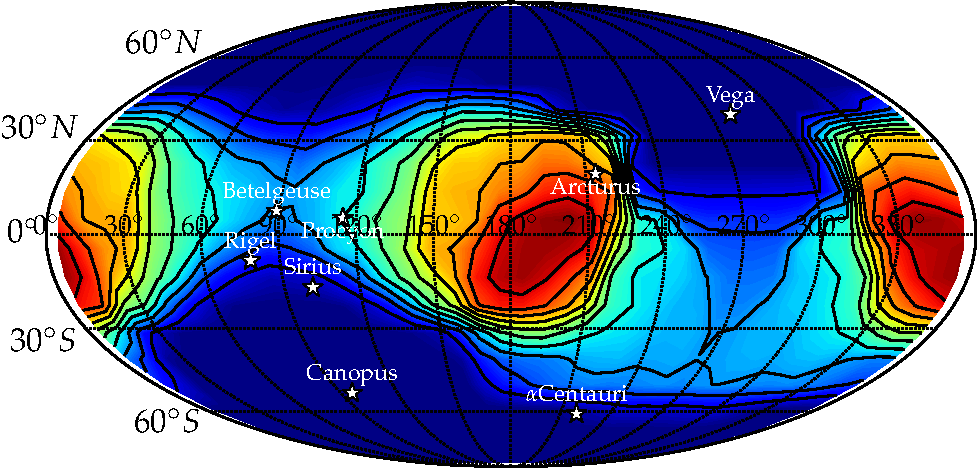
\includegraphics[width=0.6\linewidth]{700_50_mag_125_SAA}
    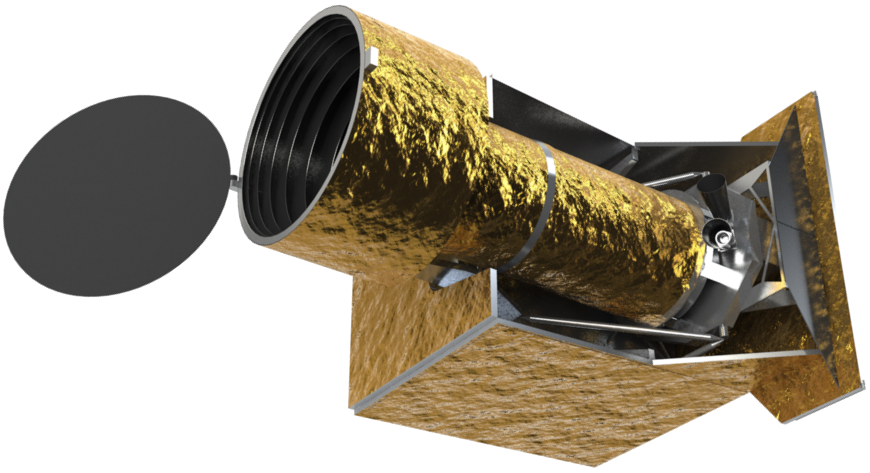
\includegraphics[width=0.2\linewidth]{instrument_large_rot.png}
  \vspace{2cm}\\
}
\author{Thibault Kuntzer\footnote{\mail{thibault.kuntzer@epfl.ch}}\ \ \& Andrea Fortier\footnote{\mail{andrea.fortier@space.unibe.ch}}}
\date{Version 1 Revision 0 -- \today}

\begin{document}

\maketitle


\clearpage

\emph{Cover image: computer rendering of CHEOPS instrument pointing towards a cumulative observation map for faint stars.}
\vspace{2em}
\tableofcontents


\section{Scope} \label{sec:scope}
Solar photons travel to Earth surface and may be reflected off the surface of the Earth back to space. Space-borne observatory that are bounded to an orbit around the Earth will be contaminated by this \emph{Earth stray light} radiation. The amount of such radiation received by an optical detector onboard the observatory will vary with time according to several criteria that correlate notably with the chosen orbit, the period of the year, the design of the telescope itself and the pointing of the satellite. 
\paragraph{}
The goal of this code is to get a first-order approximation of the Earth stray light contamination for space-borne instrument design in the first step of the mission. This tool was -- and still is -- developed to assess whether the design of an instrument could enable a photometric mission to observe faint stars ($M_V\sim12$) for a long period of time and on a spatially large field. 
More information on this exoplanet CHEOPS mission is available in \S\ref{sec:CHEOPS}. This code and the analysis tools provided are therefore influenced by the task that are at hand. It is designed in a very modular way which enables the user to develop new modules that fit his needs. 
In its current version, the scope of the code extends from the simulation of the stray light contamination to its analysis in terms of ``observable'' sky. The definition of observable is given by criteria on the available time and the deepest measurable magnitude.
\paragraph{}
This software is not designed as stand-alone analysis tool of this particular aspect of the mission. It needs to be fed with the trajectory of the satellite throughout the epoch (hence enabling complex orbits) as well as the position of the Sun during this period. Those files can be obtained by dedicated software. 
The CHEOPS orbit was generated using the commercial \verb=STK= software from company AGI. A satellite orbiting the Earth -- especially Low-Earth Orbit (LEO) -- can only observe some regions in the sky due to the presence of the Earth itself and is also limited by the presence of the Moon or other bright object in the field. The ``allowed'' region (or absolute or raw observation maps) were must also be computed beforehand. 
In the case of CHEOPS, this was done using an ad hoc \verb=MATLAB= script. The transmission of a given photon entering the telescope off-axis is characterised by a axisymmetric function about the line of sight: the Point Source Transmittance (PST). This important function depends on the exact design of the telescope and requires particular attention. Several commercial software are available to compute the PST of a given design. 
A satellite may have period during which it is unable to observe -- due for example of the presence of the South Atlantic Anomaly (SAA) -- hence another table describing shutdown phases must be provided. The European Space Agency (ESA) built a tool -- Spenvis -- that can create such tables.

As it was already mentioned, this must be seen as a first approximation software for worst case scenario, because of a simplification: the albedo of the Earth. The exact amount of photon reflected off the surface of the Earth depend on the type of material making up -- or covering -- the surface as well as on the weather. Around the poles, the albedo is higher due to the ice and the snow (around 0.9) while oceans or continents have a much lower albedo (down to 0.1) \citep{Pater2001}. In the code, the Earth is considered as a perfect sphere with an albedo of 1. This choice was made to (i) greatly simplify the code, (ii) the weather is impossible to include in this simulation and (3) the worst case estimate is wanted here. Other limitations are that only \emph{Earth} stray light is included there is no consideration of the radiation due to the Moon or any other body. The cycle of the Sun is not included in the software, but this is far from being a first-order or even a second-order 
effect.
\paragraph{}
The output of this code are as follow:
\begin{itemize}
 \item A file per minute per orbit with the table of observable region in the sky and the corresponding stray light value;
 \item Statistics files about the simulations;
 \item Error analysis of adaptive orbit step (see \ref{sec:Usage:Methods});
 \item Analysis of the mean and the maximum stray light flux;
 \item Movie of the evolution of stray light and corresponding deepest magnitude observable on short time scale;
 \item Movie of available zone in the sky versus a minimum stray light exclusion angle (see \ref{sec:Usage:Methods});
 \item Observation capabilities on the sky summed over the whole epoch according to observation rules;
 \item Prediction tables of observability of given target in the sky (beta version);
 \item Planet transit detection probabilities over the whole epoch.
\end{itemize}

\paragraph{}
The purpose of this document is to explain the usage of SALSA. \S\ref{sec:Installation} describes the installation process, \S\ref{sec:Usage} shows how to use the present code, which was used for a LEO exoplanet transit observation mission -- CHEOPS. The results of this study are summarised in \S\ref{sec:CHEOPS}. \S\ref{sec:Troubleshooting} is an attempt at troubleshooting problems the user could encounter while \S\ref{sec:KnownIssues} lists the known issues of the current version.

\section{Installation} \label{sec:Installation}
\subsection{Download}
SALSA can be downloaded from its GitHub repository: https://github.com/kuntzer/SALSA-public.
\subsection{External Dependencies}
The following software and packages are required for the code to run smoothly, so make sure they are installed before starting the simulations or the analysis. The executables for these external dependencies must all be located in your \verb=PATH=. 
\begin{itemize}
 \item Python
 \begin{itemize}
  \item Numpy (version $\geq 1.7$) \& SciPy (\httplink{http://www.scipy.org/})
  \item MatPlotLib (\httplink{http://matplotlib.org/})
  \item Basemap (\httplink{http://matplotlib.org/basemap/})
 \end{itemize}
  \item \LaTeX\ (including \verb=texlive-latex-base= and \verb=texlive-fonts-recommended=)
  \item \verb=gfortran=
  \item \verb=epstopdf= for fancy plots.
  \item \verb=pdfcrop= for fancy plots.
\end{itemize}
\subsection{Required Data}
As treated in \S\ref{sec:scope}, the code is not thought as stand-alone. It necessitate data on the satellite and on its orbit to work. The following lists the required files as well as their format and how they could be generated. In the following \verb=<id>= is an integer indexing the trajectory of the satellite and \verb=<k>= is a free integer variable describing an indexation.

\begin{description}
\item [PIPELINE]
 \item [p1 - Trajectory of the satellite] \verb=orbit_<id>.dat=
 	\\ Description: Table containing the position of the satellite with respect with the centre of the Earth.
	\\ Format: $t\ x_\text{sat}\ y_\text{sat}\ z_\text{sat}$ (blank space separators)
	\\ Units: $t$ [minutes] from the beginning of the epoch, $x_\text{sat}\ y_\text{sat}\ z_\text{sat}$ [km].
	\\ Generation: \verb=STK= (\httplink{http://www.agi.com/})
 \item [p2 - Position of the Sun] \verb=sun_<id>.dat=
 	\\ Description: Table containing the position of the Sun with respect with the centre of the satellite.
	\\ Format: $t\ x_\odot^{(\text{sat})}\ y_\odot^{(\text{sat})}\ z_\odot^{(\text{sat})}$ (blank space separators)
	\\ Units: $t$ [minutes] from the beginning of the epoch, $x_\odot^{(\text{sat})}\ y_\odot^{(\text{sat})}\ z_\odot^{(\text{sat})}$ [km].
	\\ Generation: \verb=STK= (\httplink{http://www.agi.com/})
 \item [p3 - Raw Observable Maps] \verb=raw_maps_<id>/orbit_<k>.dat=
 	\\ Description: Tables containing the allowed observation regions (cells of a grid) in the sky per one orbit and per minute. $k$ runs on all orbits.
	\\ Format: $t,\alpha,\delta$
	\\ Units: $t$ [minutes] from the beginning of the epoch, $\alpha$ (right ascension), $\delta$ (declination) [rad].
	\\ Generation: Ad hoc software that takes into account the constraints (SL exclusion angle, Moon exclusion angle, Solar system bodies, \dots) on the observations.
\item [p4 - PST] \verb=pst.dat=
 	\\ Description: Table of the PST values.
	\\ Format: $\theta\quad PST$
	\\ Units: $\theta$ [degree], $PST$ [-]
	\\ Generation: Ad hoc software such as \verb=Zeemax= or \verb=TracePro=.
\item [ANALYSIS TOOLS]
\item [a1 - Index of the Orbits] \verb=minute_table_<id>.dat=
 	\\ Description: Contains a conversion table between orbit $k$ and start and stop time stamps. The keyword \verb=rel= means time since the beginning of the current orbit while \verb=abs= since the beginning of the epoch. Hence $t_\text{rel}$ runs from 0 to one period.
	\\ Format: $k_\text{orbit},t_\text{start,rel},t_\text{start,abs}$ [new line] $k_\text{orbit},t_\text{stop,rel},t_\text{stop,abs}$
	\\ Units: $k_\text{orbit}$ [-], $t$ [min]
	\\ Generation: Ad hoc script that analyses \verb=orbit_<id>.dat=.
\item [a2 - Shutdown Events] \verb=SAA_table_<id>.dat=
 	\\ Description: Describes when the observations are not possible (notably when over the South Atlantic Anomaly -- SAA).
	\\ Format: $t_\text{start},1$[new line]$t_\text{stop},0$
	\\ Units: $t_\text{start}, t_\text{stop}$ [min]
	\\ Generation: ESA tool Spenvis \httplink{http://www.spenvis.oma.be/}
\item [a3 - Position of the Moon] \verb=moon_<id>.dat=
 	\\ Description: Table containing the position of the Moon with respect with the centre of the satellite.
	\\ Format: $t\ x_m^{(\text{sat})}\ y_m^{(\text{sat})}\ z_m^{(\text{sat})}$ (blank space separators)
	\\ Units: $t$ [minutes] from the beginning of the epoch, $x_m^{(\text{sat})}\ y_m^{(\text{sat})}\ z_m^{(\text{sat})}$ [km].
	\\ Generation: \verb=STK= (\httplink{http://www.agi.com/})
\end{description}

\subsection{Setup} \label{sec:setup}
The complete code can be seen as two separate codes. The first part is called \emph{pipeline} in the following during which the stray light flux on the detector is computed. The second part is the analysis (\emph{Analysis Tools}) of the simulated stray light flux. They can be run only sequentially which increase modularity at the cost of increasing the required time. Therefore, the pipeline can be set up separately from the analysis tools. They both require some common libraries as well as several strictly-organised software. The version downloaded should already contain a working folder tree.

\subsubsection{Pipeline}
Several instances of the pipeline can be run simultaneously. Therefore, for the pipeline only, a variable \verb=part/p= is added. 
The situation can be summarised as follow (with \verb=id= the orbit id, \verb=SL= the SL exclusion angle, \verb=p= the CPU number):
\begin{figure*}[h]
\begin{center}
% Define block styles

\tikzstyle{decision} = [diamond, draw, fill=gray!20, text width=4.5em, text badly centered, node distance=2.cm, inner sep=0pt]
\tikzstyle{block} = [rectangle, draw, text width=8em, rounded corners, minimum height=2em, node distance=3.5cm]
\tikzstyle{algo} = [rectangle, draw, fill=gray!20, text width=5em, node distance=1.5cm]
\tikzstyle{algolarge} = [rectangle, draw, fill=gray!20, text width=7em, node distance=2.5cm]
\tikzstyle{algoverylarge} = [rectangle, draw, fill=gray!20, text width=10em, node distance=2.5cm]
\tikzstyle{code} = [rectangle, draw, fill=red!20, text width=7em, text centered, rounded corners, minimum height=3em, node distance=3.5cm]
\tikzstyle{line} = [draw, -latex']
\tikzstyle{cloud} = [draw, ellipse, text width=5em]
   
  
% \resizebox{!}{1\textwidth}{%{1\textwidth}{
\begin{tikzpicture}[scale=2, node distance = 2.5cm, auto]
  \node [code] (raw_maps) {\verb=raw_maps_=\\\verb=<id>/=};
  \node [code, left of=raw_maps] (resources) {\verb=resources/=};
  \node [code, right of=raw_maps] (sl_code) {\verb=stray_light=\\\verb=_<id>_<p>/=};
  \node [code, right of=sl_code] (results) {\verb=<id>_<p>/=};
%   \node [block, right of=sl_code] (compute) {\verb=1-compute=\\\verb=_<id>_<p>.py=};
  \node [block, right of=results] (param) {\verb=parameters.py=};
  
    \node [code, below left of=sl_code] (1) {\verb=INPUT/=};
  \node [code, left of=1] (2) {\verb=CODE/=};
  \node [code, below right of=sl_code] (3) {\verb=ORBIT/=};
  \node [code, right of=3] (4) {\verb=OUTPUT/=};
  
  \node [block, below of=2] (5) {SL code};
  
  \node [block, below of=1] (8) {\verb=pst.dat=};
  
  \node [block, below right of=3] (7) {\verb=sun_<id>.dat=};
  \node [block, left of=7] (6) {\verb=orbit_<id>.dat=};
  
  \path [line] (sl_code)--(1);
  \path [line] (sl_code)--(2);
  \path [line] (sl_code)--(3);
  \path [line] (sl_code)--(4);
  \path [line] (2)--(5);
  
  \path [line] (3)--(7);
  \path [line] (3)--(6);
  
  \path [line] (1)--(8);

\end{tikzpicture}
% }
\caption{Flow chart of the different folders in the pipeline folder. The folder raw\_maps\_<id>/ contains in addition the files p3 deg/orbit\_<k>.dat. The list of for the folder resources is available in the following. The folders <id>\_<p>/ will contain the results of the simulation.\label{fig:folder-tree-pipeline}}

\end{center}
\end{figure*}

In the \verb=resources/= folder, the following files are required:
\begin{itemize}
 \item \verb=minute_table_<id>.dat=
  \item \verb=sun_<id>.dat=
  \item \verb=moon_<id>.dat=
  \item \verb=orbit_<id>.dat=
  \item \verb=saa_table_<id>.dat=
\end{itemize}
To adjust the wavelengths of the instrument of the satellite, the Solar constant in this band must be modified in \verb=constants= while the pixel size and the minimal SL exclusion angles must be given in \verb=parameters=. Other characteristics of the detector must be entered in \verb=parameters.py= in the root directory. Those include:
\begin{itemize}
 \item \verb=radius_psf= The size of the PSF in pixel
 \item \verb=radius_tele= The radius of the telescope in metres
 \item \verb=dlambda_over_lambda= the factor $\frac{\delta\lambda}{\lambda}$ (See \S\ref{sec:numerics-functions} for more information).
\end{itemize}
One important parameter must be set up in the \verb=straylight_<id>_<p>/CODE/parameter= file :
\begin{itemize}
 \item \verb=pixel= which is the pixel size in cm$^2$.
\end{itemize}
Further parameters control debugging functions and should be self-explanatory. A grid representing the Earth of at least $1001\times 501$ is required. This is needed for the simulations to converge to a good estimation of the flux. 

\subsubsection{Analysis Tools}
There, at least the following three folders must exists:
\begin{itemize}
 \item \verb=<id>_figures/= contains all the figures generated
 \item \verb=<id>_flux/= contains all the flux data generated by the pipeline
 \item \verb=<id>_misc/= contains all data generated by the analysis
\end{itemize}
In addition, the file \verb=parameters.py= must contain the following information:
\begin{itemize}
 \item \verb=last_orbits= a Python dictionary \verb=<id>:<last orbit>=
 \item \verb=ppm_threshold= the minimum SNR acceptable in ppm.
 \item \verb=resx,resy= the resolution of the rectangular sky grid.
  \item \verb=mirror_efficiency= the efficiency of the optical system. I.e. the ratio of photons reaching the detector by the number of photons entering the optical system.
 \item \verb=SL_post_treat_reduction= efficiency of the stray light removal algorithm in the data reduction pipeline.
\end{itemize}
The other options are optional and self-explanatory. Further setup of the analysis tools are described in each module. In \verb=resources/constants.py=, there are definitions of the wavelengths used:
\begin{itemize}
 \item \verb=wavelenght_visual=
 \item \verb=Fv=
 \item \verb=Jy=
\end{itemize}
For more information about the variables, refer to \ref{sec:numerics-functions}.


\section{Numerical Methods}\label{sec:Usage:Methods}
In this section, the algorithms and the softwares used and prepared are presented. The presentation starts by discussing the calculation of the visible area that was coded by Luzius Kronig from EPFL/Swiss Space Center, continues by describing the stray light code of Andrea Fortier at Unibe and Thibault Kuntzer and ends by the description of the various algorithms and techniques developed to derive stray light maps and tables. A flow chart summarises the numerical codes used in Fig. \ref{fig:data-flow}.
\begin{figure*}
\begin{center}
% Define block styles
%\tikzstyle{decision} = [diamond, draw, fill=blue!20, text width=4.5em, text badly centered, node distance=3cm, inner sep=0pt]
\tikzstyle{decision} = [diamond, draw, fill=gray!20, text width=4.5em, text badly centered, node distance=2.cm, inner sep=0pt]
\tikzstyle{block} = [rectangle, draw, text width=7.5em, rounded corners, minimum height=2em, node distance=3.5cm]
\tikzstyle{algo} = [rectangle, draw, fill=gray!20, text width=5em, node distance=1.5cm]
\tikzstyle{algolarge} = [rectangle, draw, fill=gray!20, text width=7em, node distance=2.5cm]
\tikzstyle{algoverylarge} = [rectangle, draw, fill=gray!20, text width=10em, node distance=2.5cm]
\tikzstyle{code} = [rectangle, draw, fill=red!20, text width=5em, text centered, rounded corners, minimum height=5em, node distance=2.5cm]
\tikzstyle{line} = [draw, -latex']
\tikzstyle{cloud} = [draw, ellipse, text width=5em]
   
\resizebox{!}{1\textwidth}{
\begin{tikzpicture}[scale=2, node distance = 2.5cm, auto]
  \node [block] (raw_maps) {Observable\\regions};
  \node [block, left of=raw_maps] (constraints) {Constraints\\\textbullet\ Sun\\\textbullet\ Earth\\\textbullet\ SL angle\\\textbullet\ Moon};
  \node [block, right of=raw_maps] (stk) {STK Simulator\\\textbullet\ Orbit\\\textbullet\ Sun \\ \textbullet\ Moon};
  \node [code, below of=raw_maps] (sl) {Stray light pipeline\\\S\ref{numercis:stray_light.f} \& \ref{sec:numerics-pipeline}};
  \node [block, right of=sl] (tolerance) {\textbullet\ Tolerance $\epsilon$\\\textbullet\ Orbit\\\textbullet\ Sun};
  \node [algo, below of=sl] (orbit_0) {$i:=1$};
  \node [algo, below of=orbit_0] (orbit_i) {Compute orbit $i$};
  
  \node [algoverylarge, left of=orbit_0, node distance=6cm] (for) {\emph{for every minutes:}};
  \node [algoverylarge, below of=for, node distance=1cm] (c1) {Day/night on Earth};
  \node [algoverylarge, below of=c1, node distance=1cm] (c2) {Illumination gradient};
  \node [algoverylarge, below of=c2, node distance=1cm] (c3) {$\oplus$ surface seen by sat.};
  \node [algoverylarge, below of=c3, node distance=1cm] (c4) {\emph{for every visible point:}};
  \node [algoverylarge, below of=c4, node distance=1cm] (c5) {Contributing surfaces};
  \node [algoverylarge, below of=c5, node distance=1cm] (c6) {Convolve photons flux by PST};
  
  
  \node [algo, below of=orbit_i] (orbit_next) {Compute orbit $i+\Delta i$};
  \node [decision, below of=orbit_next] (step) {$\max \Delta <\epsilon$};
  \node [algolarge, below left of=step] (go) {$\Delta i:=
  \begin{cases}2\Delta i&\textcircled{a}\\
	      \Delta i&\textcircled{b}
	      \end{cases}$};
  \node [algolarge, below right of=step] (nogo) {$\Delta i:=\begin{cases}\frac{\Delta i}{2} & \textcircled{c}\\1& \textcircled{d}\end{cases}$};
  \node [decision, below left of=nogo, node distance=2.5cm] (imax) {$i+\Delta i>i_{\max}$};
  \node [algo, right of=imax, node distance=4.5cm] (iplus) {$i:=i+\Delta i$};
  \node [code, below of=imax, node distance=3cm] (analysis) {Stray light analysis\\ \S\ref{sec:numerics-analysis}};
  \node [block, right of=analysis] (params) {\textbullet\ range mag\\\textbullet\ PSF\\\textbullet\ $t,t_\text{obs}$\\\textbullet\ \dots};
  \node [block, below of=analysis, below of=analysis, node distance=1.2cm] (A) {Sky maps of stray light};
  \node [block, left of=A] (B) {Stray light flux variations};
  \node [block, left of=B] (C) {Orbits \& error evolution};
  \node [block, right of=A] (D) {Maps cumulative exposure};
  \node [block, right of=D] (E) {Planning \& transit detection};


   \path [line] (constraints)--(raw_maps);
   \path [line] (stk)--(raw_maps);
   \path [line] (raw_maps)--(sl);
   
   \path [line] (sl) -- (orbit_0);
   \path [line] (tolerance)--(sl);
   \path [line] (orbit_0) -- (orbit_i);
   \path [line] (orbit_i) -- (orbit_next);
   
   \path [line] (orbit_i.west) -- (for.east);
   \path [line] (for) to (c1);
   \path [line] (c1) to (c2);
   \path [line] (c2) to (c3);
   \path [line] (c3) to (c4);
   \path [line] (c4) to (c5);
   \path [line] (c5) to (c6);
   \path [line] (c6.east) to (orbit_i.west);
   
   \path [line] (orbit_next) -- (step);
   \path [line] (step) -- node {yes} (go);
   \path [line] (step) -- node {no} (nogo);
   \path [line] (go) -- (imax);
   \path [line] (nogo) -- (imax);
   \path [line] (imax) -- node {no} (iplus);
   \path [line] (iplus.north) to (orbit_i.east);
   \path [line] (imax.south) to node {yes} (analysis);
    \path [line] (params) -- (analysis) ;

    \path [line] (analysis.south) to (A);
    \path [line] (analysis.south) to (B);
    \path [line] (analysis.south) to (C);
    \path [line] (analysis.south) to (D);
    \path [line] (analysis.south) to (E);
\end{tikzpicture}
}
\caption{Flow chart of the project. Red blocks represent the different code suites used in this project. Gray cells depict algorithmic instructions and white either inputs or outputs of the project. \label{fig:data-flow} STK is the commercial software used to generate the orbit of the satellite. $i$ is the orbit number, $\Delta i$ represent the orbit step size and $i_{\max}$. $\max\Delta$ is the maximal (relative) difference in the equivalent magnitude. The conditions on the orbit step size are $\textcircled{a}$ if $\Delta i$ is smaller than a maximum orbit size; $\textcircled{b}$ else; $\textcircled{c}$ if $\frac{\Delta i}{2}\geq 1$; $\textcircled{d}$ else.}
\end{center}
\end{figure*}
\subsection{Observable Area} \label{sec:numerics-obs}
An visible region in the sky is an area that the satellite can observe at a given time. The geometry of this zone is primarily defined by the position of the satellite relative to objects that could contaminate the image either by direct imaging or by diffuse light such stray or zodical lights. Most of the constraints are therefore derived from the pointing direction -- the line of sight -- of the telescope. This paragraph describes quickly the steps leading to the computation of observable sky.
\paragraph{Constraints} \label{sec:numerics-visibility-constraints}
\begin{wrapfigure}{r}{0.45\textwidth}
 \begin{center}
  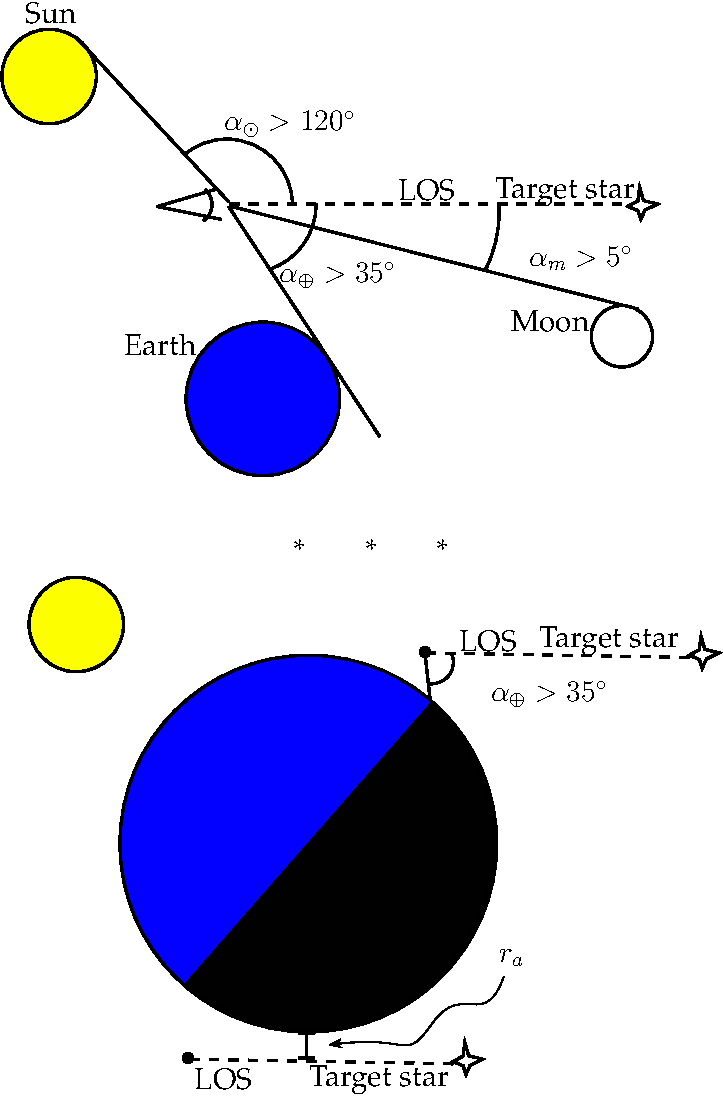
\includegraphics[width=1\linewidth]{exclusion-angles}
    \caption{\emph{Top}. Exclusion angles from the line of sight (LOS) of the telescope. \emph{Bottom.} Close-up for different cases for observations above the dark side of the Earth. All values refer to the CHEOPS mission.}
    \vspace{-5em}
  \label{fig:exclusion-angles}
 \end{center}
\end{wrapfigure}
The first constraints on this area are that it is forbidden to look directly at or close to bright objects namely the Sun, the Earth and the Moon. Moreover, to reduce the contamination by diffuse light of the Sun or Earth and Moon stray lights, there are conditions on the minimum angles between the line of sight (LOS) of the telescope and the limb of those objects. 
\begin{description}
 \item [Earth Occultation] The telescope shall not point to a target, which projected altitude from the surface of Earth is less than 100 km (thickness of the Earth's atmosphere);
 \item [Earth stray light exclusion angle] In order to limit stray light contamination, the minimum angle allowed between the line of sight and any (visible) illuminated part of the Earth limb, the so-called Earth stray light exclusion angle shall be $\alpha_\oplus$;
 \item [Sun exclusion half-angle] The Sun must be outside the cone around the line of sight (LOS) of the telescope having a half-angle, the so-called sun exclusion angle, of $\alpha_\odot$;
 \item [Moon exclusion half-angle] The bright Moon must not be inside a cone around the line-of-sight of the
telescope having a half-angle, the so-called moon exclusion angle, of $\alpha_m$.
\end{description}
The constraints shape the observable regions; figure \ref{fig:exclusion-angles} depicts those exclusion angles for CHEOPS.

The South Atlantic Anomaly (SAA) plays also an important role as crossing it requires instrument shutdown.

The maps of the visible regions in the sky are generated without taking the SAA into account and the restriction is applied afterwards during the analysis. Otherwise, if the SAA would already be included in the observability maps, it would be impossible to perform an adaptive orbit step as described in the next section. Indeed, the crossing of the SAA does not always occur at the same time in the orbit. Moreover, the time spent over the SAA changes as well.

\paragraph{Coordinate System.} The observable region in the sky must be in reference to the satellite. To describe the system (Sun, Earth, Moon, satellite) a common coordinate system must be chosen. The chosen frame is the International Celestial Reference Frame (ICRF). In order to perform the computations, the centre of this coordinate system is translated into the satellite. Therefore, all positions are translated to the satellite and not the Earth.
\paragraph{Discretisation in Space.}
The sky is simulated by a grid of points described by the following relationships:
\begin{eqnarray}
%\begin{array}{l}
\alpha_g(i) = \frac{\Delta \alpha}{2}+i\Delta\alpha,\ i=\{0,\dots,n-1\} \nonumber\\ % \in [0,2\pi] 
\delta_g(j) = -\frac{\pi}{2} + \frac{\Delta \delta}{2}+j\Delta\delta,\ j=\{0,\dots,m-1\} %  \in [-\frac{\pi}{2},\frac{\pi}{2}]
%\end{array} 
\label{eq:grid}
\end{eqnarray}
where $n,m$ describe the resolution of the gird. This grid yield cells on the sky of $\Delta \alpha \times \Delta \delta$ or $9^\circ \times 9^\circ$. Fairly large cell are to be used. It arises from the computation time of the different steps which scales at least as $\mathcal{O}(n\cdot m)$.

\paragraph{Discretisation in Time.}
The orbital period of the satellite depends of course on the altitude following the famous third Kepler law:
$$ P = 2\pi \sqrt{\frac{a^3}{Gm_\oplus}} $$
The observability maps will be used to plan the observation and therefore, it is better to have a time in minute rather than the position in a given orbit. The time $t_0=0$ min is the beginning of the epoch.

\paragraph{Outputs} 
The output files must be a list of the right ascension $\alpha$ and the declination $\delta$ of the grid points which are observable. In order to reduce the number of files generated, the visible points are all grouped in one single file for one orbit. Hence, the final output files are given in the following format : \verb=t, ra, dec= in, respectively, minutes and radians.
\subsection{Stray Light Code} \label{numercis:stray_light.f}
To compute the Earth stray light that enters the telescope and hit the detector, a dedicated code in \verb=Fortran= was designed by Andrea Fortier and Thibault Kuntzer. This program named \verb=stray_light.f= can compute independently of the observability map code, the stray light contamination at any time and in any direction. 


\paragraph{The Steps to Stray Light Evaluation.}
The stray light computation is divided in several steps:
\begin{enumerate}
 \item Compute the illuminated part of the Earth;
 \item Compute the gradient of the illumination;
 \item Compute which parts of the illuminated Earth are visible by the telescope;
 \item For every visible region or ``targets'', do the following:
 \begin{enumerate}
  \item Compute the flux of light reflecting off Earth's surface that reaches the telescope;
 \item Convolve this signal by the PST to get the flux of Earth stray light at the detector.
 \end{enumerate}
\end{enumerate}
Those steps are explained in further details below. It is necessary to caution the reader that the description of the process is very linear here and does not exactly mirror the implementation in which numerical optimisation was planned. 
\paragraph{}
In the software, a few simplifications are made: Firstly, only the \emph{Earth} stray light is computed. Contamination from the Moon is not considered as it is assumed that its exclusion angle is sufficient. Secondly, the Earth is considered to be a perfect sphere thus neglecting its bulge and hence slightly miscalculating the off-axis angle of an incoming photon. 
The surface of this sphere is supposed to be uniform: no distinction is made between oceans or land, the weather is not simulated (therefore thunderstorms and aurorae are not considered) and cities not modelled. To get a upper estimate of the stray light, the albedo of the Earth is set to 1. The albedo is a multiplicative factor in the calculation of the flux (See \S\ref{sec:numerics-functions} for more details). The value of the averaged albedo ($\sim$ 0.3 -- 0.5) on the Earth could therefore be used. 
However, it was chosen to set the albedo to 1 to compute a worst case scenario, but with little difference to a finely tuned value because of the logarithmic behaviour of the final output of the project (as discussed in \S\ref{sec:KnownIssues}).

\paragraph{Illuminated Earth.}
The first step is to describe with enough precision the illuminated part of the Earth. The only interesting part of the Earth at this point is the one in daylight. Indeed, it is considered that half of the Earth which is the night does not contributed to stray light.There are thunderstorms, aura or even city lights that could contaminate the signal if the LOS were too close to the limb of the Earth. 
Those effects which are extremely complex to simulate are not integrated in the code, but the constraint to point above the atmosphere with a given minimal altitude used to ensure that there is no contamination.

The surface of the Earth is represented by a grid for which every cell is determined to be either in the day or in the night depending on the dot product of its normal and the direction of the Sun. The minimum grid that can achieve sufficient accuracy, \emph{i.e.} that the flux of stray light has converged, is quite large with 1000 by 500 cells.

\paragraph{Illumination Gradient.}
For the cells that are in the sunlight, the intensity $I$ of the light is computed by determining the cosine of the angle at which the light impacts the cell $c$. This depends upon the relative position of the cell and the Sun and can be computed using the following formula:
\begin{equation}
 I_c \propto \cos \varphi
\end{equation}
where $\varphi$ is the angle between the direction of the Sun and the normal vector of the cell (See \S\ref{app:great-circle-distance}).
The amount of radiation that arrives at a particular cell is also given by the energy received by the Sun at the distance of the orbit of the Earth. Here, the common value of about 1360 W/m$^2$ is not considered as it takes the whole spectrum into account. The solar constant must be reduced to the applicable band window. For example, CHEOPS instrument is sensitive to the range of wavelengths from 400 to 1100 nm and the solar ``constant'' for this interval can be computed to be 880 W/m$^2$. 

\paragraph{Changing Viewpoints.}
The two previous parts can be carried out without the knowledge of the orbit at that particular time. Indeed, the satellite plays no role. This step determines which illuminated cells can be seen by the satellite at any given time. Assuming a position for the satellite, the code finds all cells within a cone defined by all visible tangent directions on the surface of the Earth and flags them as relevant to the stray light computation. See figure \ref{fig:numerics-illuminated-earth} for an example.

\begin{figure}[!h]
 \begin{center}
  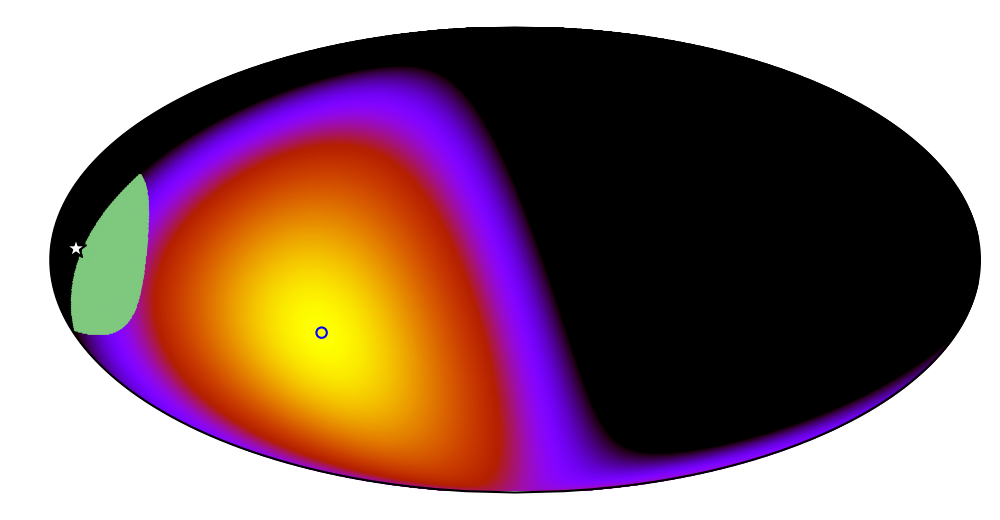
\includegraphics[width=0.6\linewidth]{map-2}
  \caption{Mollweide projection of the illuminated Earth. The circle on top of the maximal illuminated region is the projection of the position of the Sun, the white star-shaped marker symbolises the satellite and the green region is the illuminated Earth seen by the satellite.\label{fig:numerics-illuminated-earth}}
 \end{center}
\end{figure}


\paragraph{Flux of Photons at the Telescope.} The flux of photons at the entrance of the telescope (not at the detector or somewhere else in the optical path) depends upon the direction of the line of sight. Let $\theta$ be the angle between the LOS and the photon path. The target star is denoted by $\pmb{r}_\star$, the position of the satellite by $\pmb{r}_s$ the cell position by $\pmb{r}_c$ all with reference to the centre of the Earth. The direction to which the photon bounced off the cell to the satellite can be defined by the vector $\pmb{v} = \pmb{r}_s-\pmb{r}_c$. If the angle $\theta$ is larger than $\pi/2$, then no photons will hit the telescope:
\begin{eqnarray}
\pmb{r}_\star\cdot \pmb{r} =  |\pmb{r}_\star|\cdot |\pmb{r}|\cos\theta \\
\nonumber\\ 
 \cos \theta = \begin{cases} >0&\text{No hit} \\ \leq 0 & \text{photon hit} \end{cases}
\end{eqnarray}
To obtain the value of the total flux of photons all that is left is to integrate on all possible directions. The surface of the Earth is assumed to be Lambertian\footnote{A Lambertian surface is a surface whose radiance (power per unit solid angle per unit projected source area) is the same independently of the angle of view. Its apparent brightness is the same.}. This is justified as the albedo is assumed to be constant and because the radiant intensity (power per unit solid angle) depends upon the cosine of the angle described by the direction of the radiation leaving the point. The same cosine factor is applied to the surface that emits the radiation and therefore they cancel out.

\paragraph{Accounting for the Photon Rejection.} Up until this point, the considerations were mostly geometrical. The Earth is assumed to be a perfect sphere which reflects light with the same radiance in any direction. The cells that can be seen by the satellite are defined by its orbit. Hence computing the angles from the LOS to them is easy.
So, at this point in the code, the amount of photons reaching the pupil of the telescope is computed each with an off-axis angle $\theta$. The transmission of the incoming photons through the telescope can be approximated by a axisymmetric function that depends upon the off-axis angle $\theta$ of the radiation : the point source transmission (PST) -- See for example \cite{Breault2010} or \cite{Pompea1995}. 
The energy that arrives at the detector is multiplied by the value of the PST as function of the off-axis angle of the photon. 
An interpolation of the PST is performed to fill the gaps in the knowledge of this function which is sampled using large steps. The flux is also converted to photons per second per pixel. As the stray light is scattered by different parts of the telescope and not through the optical path of the mirrors and focal planes, its signal is not convolved by the PSF and hits a single pixel.

\paragraph{Practicalities.} The code was optimised to perform stray light computations for known observability maps and ephemerides for the Sun. It takes as input parameters a PST (\verb=theta [deg],PST=), the position of the satellite (in the frame of reference of the Earth) and the Sun in separate file containing \verb=x,y,z,ra,dec,r= with distances in km and angles in radians. Finally two files describe the target list: one containing the number of targets to optimise the \verb=Fortran= memory management and file handling and a list of targets with two columns: the right ascension and the declination both in radians. 

\subsection{A Pipeline to Compute the Stray Light Flux} \label{sec:numerics-pipeline}
To generate a stray light map of the observable sky at a given time, a \verb=Python= script looks for the corresponding observability map, creates the list of visible points which are then given as inputs to the stray light calculator along with a few other variables (position of the Sun and the Earth, \dots) as described in section \S\ref{numercis:stray_light.f}. To speed up computation, an adaptive time step is implemented. An orbit is computed every minute, however as there are around 15 orbits per day in LEO, consecutive orbits are very similar in most of the cases. Hence the capability of skipping orbits that are too similar. This is done by computing orbit $i$ and then orbit $i+10$. If the comparison of the two orbits $(i, i+\Delta i)$ reveals a difference of more than 5\% in stray light flux, then the orbit $i+\Delta i/2$ is computed. Those parameters can be changed. 
The algorithm always tries to increase the number of step and doubles the step size if it is (1) smaller than the optimum and (2) the error to the previous orbit is less than the threshold. The maximum bearable error to the next step can be chosen such that it would ensure that the \emph{maximal} error in the orbit in term of equivalent magnitude (see \S\ref{sec:numerics-functions}). 

This step of generating stray light maps for the whole epoch is the most lengthy one. The time needed to compute a whole year with the adaptive orbit step described in the above depends on the altitude as the stray light is less prominent at high altitude. The outputs are one file per minute containing the following characteristics: time, grid point position in radians (right ascension, declination) and the flux of stray light in ph px$^{-1}$ s$^{-1}$. The relative high number of output files ($\sim 5-10\cdot 10^5$) weight around 1--2 GB and will be analysed in the next steps for a whole year.
The temporal resolution is chosen to be the same as the observability maps.

\subsection{Analysis of Stray Light Data} \label{sec:numerics-analysis}
To interpret the data, several analysis tools were developed. The scripts range from the very simple counting of computed orbits to a much more elaborated probability of observing a transit estimation. A description of some of those tools is provided here. 
\paragraph{Computed Orbits.} This is the first logical step -- compulsory in order to proceed to other functions --: check which orbits have been computed. This seems redundant as this list can easily be retrieved from logging at the previous step when computing the stray light maps. In order to speed up the computations, most of the stray light data can be generated with several CPUs: not in parallel, but working on different periods in the epoch. To avoid any mistake when merging back the results of the different CPUs, this scripts tests if minutes 0, 20 and 60 were computed. As the SAA (shutdown periods) is not considered, each of those minutes had to be computed. If any fails, then it is considered that this orbit was not computed.

\paragraph{Analysis of the Error Evolution.} The second step is to check that the error from one orbit to the next is not larger than the limit or if it is, then that every orbit is computed. This operation is rather slow as the code must compare the minutes pairwise in each orbit and due to non-integer period, several combinations must be made to find the best fit. 

\paragraph{Analysis of the Stray Light Flux.} From this point forward, the data is considered as robust if the two previous steps did not pointed out to erroneous behaviours. The stray light flux depends upon the amount of Earth illuminated cells seen and their illumination. In order to characterise those changes the stray light flux is analysed by four different quantities:
\begin{enumerate}
 \item The \emph{maximal value}: the maximal value of the flux for a given orbit;
 \item The \emph{maximal mean}: taking the maximum value of the flux for one minute, repeating for every minute in the orbit and averaging;
 \item The \emph{twice-averaged mean}: taking the average of the flux at a particular moment in the orbit, repeating for every minute in the orbit and taking the average on those averages per minute;
 \item The \emph{evolution in one orbit} of the stray light in one direction.
%  \item The \emph{direction of maximal flux}: finding out which where is the .
\end{enumerate}

\paragraph{Stray Light Flux Maps.} The list of the visible targets is completed by the stray light flux. Therefore, a projection of the targets can be made on a map with a colour assigned to the stray light. A conversion to limiting magnitude can be made to represent how faint the observed stars can be given a certain SNR (see \S\ref{sec:numerics-functions}). Those maps have the advantage -- beside being aesthetically pleasant -- of showing the varying visible regions in the sky and the effect of the relative alignment of the Earth and the Sun. 
\paragraph{Cumulative Observation Maps.} The cumulative observation time is a value that is computed on a long period of time. There is a minimum of observation time to consider the observation worth it. On top of this minimal observation time, the telescope takes time to align its LOS to the star: the acquisition time.
Those maps give informations about which regions of the sky are invisible which can be observed the longest and the effects of the constraints and the SAA. Those maps are relatively long to establish as the appearance and disappearance times -- which occurs many times over the course of the year -- of every grid point must be computed.

The time of observation can be understood in different ways. We provide proposed definitions:
\begin{description}
 \item [Cumulative observation time] describes how much time can the satellite observe in one orbit whose start and ending are arbitrary defined. Interruptions in the cumulative observation time are acceptable. In this document, it is often short-handed to ``observation time''.
 \item [Consecutive observation time] describes how much time can the satellite observe without interruptions in the observations. If needed arbitrary start and ending time of the orbits can be defined.
 \item [Accumulated observation time] is the total amount of either cumulative or consecutive time. 
 \item [Period of observation] represent the number of days a target is observable. It does not describe the observable time, rather how many days the target can be followed.
\end{description}
Observation maps are produced for the two definitions (cumulative and consecutive observation time). Subtraction of two maps to see the difference between two observational strategies are  

\paragraph {Probability of transit detection} SALSA was developed for a mission which goal is to characterise planets by observing their transits. This tool aims at estimating the probabilities of transit detection given the absolute observation regions and the stray light contamination. This tool is limited to looking at the transit duration versus the effective observation possibility. It does not evaluate the possibility of detecting the transit on the basis of its depth. SALSA looks for specific transit patterns. They represent certain families of objects transiting their star. Those families have typical period of rotation and transit time \citep{redbook}. Their ingress and exgress time is supposed to be unknown. SALSA assumes that the ingress time is described by an uniform probability distribution. The next step is to find how many of those transit times per rotation around the star are visible. Depending upon the observational conditions, certain objects can be observed for more than the time between two transits and thus will have probabilities of more than one. If an object can be observed non-consecutively and the total observation time is still larger than the time between two orbits, the probability is still considered more than one.
\paragraph {Almanac of catalogs} Using a similar procedure and providing a catalog of objects, their rise and setting time in the effective observational region are computed. Such kind of data can be used for the planning of the observations. This module can then easily be turned into an observation scheduler.


\subsection{Computational Details}\label{sec:numerics-functions}
\paragraph{From Stray Light Flux to Maximum Magnitude Visible.} 
The question asked here is: given the stray light flux, what is the faintest target visible? The function \verb=flux2mag= (and the reciprocal \verb=mag2flux=) yields this limiting magnitude (or inversely the flux) of the target star. The noise represented by the stray light to the flux of the star must be at maximum $T$. The flux is related to the magnitude $m$ by:
\begin{equation}
 F = 10^{-2/5\cdot m}
\end{equation}
which has units of ergs s$^{-1}$ cm$^{-2}$. The flux of stray light is given in units of ph s$^{-1}$ px$^{-1}$. Moreover, only photons with a certain energy matter and not all the spectrum of light. Therefore the flux is now given by:
\begin{equation}
 F_\text{sl}(m_V) = \underbrace{F_V J_V\frac{\Delta \lambda}{\lambda}}_{\equiv A}\cdot\underbrace{\left(\frac{R_\text{tel}}{R_\text{PSF}}\right)^2}_{\equiv B}\cdot10^{-2/5\cdot m_V}
\end{equation}
% \todo{see: \httplink{http://astro.wku.edu/strolger/UNITS.txt}}
where $F_V = 3640$ Jy cm$^2$/ergs converts from ergs to Jansky for the band $V$, $J_V$ transforms from energy to the flux of photons for the band $V$: $J_V=1.51\cdot10^7$ photons s$^{-1}$ m$^{-2}$ / Jy. $\frac{\Delta \lambda}{\lambda}$ is the bandwidth of the instrument. Those three parameters grouped in $A$ depend upon the choice of the band. $R_\text{tel}$ is the radius of the aperture in metres. $R_\text{PSF}$ px is the radius of the PSF in pixels. The PSF is modelled here as an axisymmetric step function (top hat function) such as 
\begin{equation} \label{eq:modelled-PSF}
 \text{PSF}(r) = \begin{cases} 1 & r\leq R_\text{PSF}\\
			     0 & r>R_\text{PSF}
              \end{cases}
\end{equation}
Those two radius are geometrical parameters and their ratio squared transforms from m$^2$ to pixels and is noted for convenience $B$.

The SNR for the stray light is given by $SNR=1/T$ and therefore, the maximum stray light flux tolerable for a given magnitude is:
\begin{equation} \label{eq:num-mag2flux}
 F_\text{sl}(m_V) = T\cdot AB\cdot10^{-2/5\cdot m_V}=\frac{AB\cdot10^{-2/5\cdot m_V}}{SNR}
\end{equation}
This computation is implemented in \verb=mag2flux=. The reciprocal function uses equation \ref{eq:num-mag2flux} to express $m_V(F_\text{sl})$. This implies that there is a logarithmic of base 10 function. In order to avoid numerical errors while performing this computation, the stray light flux is clipped to a minimal value of $10^{-40}$ ph s$^{-1}$ px$^{-1}$. 

\paragraph{Comparing Two Orbits.} This function is important as it decides whether the orbit step size in the calculations of the stray light flux must be reduced. It must, therefore, read the data from the two orbits and compare them. This function is quite conservative in the sense, that it returns the \emph{maximal} difference in the orbit and not the \emph{mean}. The two orbits (the \verb=reference= and the \verb=current= as defined in the code) are compared pairwise: minute by minute. As evoked before, this is a none trivial problem as the orbital period is not an integer of minutes. Therefore, three combinations are tested using a shift $s=\{0,1,2\}$ in time between the reference and the current orbits.

\paragraph{Great Circle Distance.} \label{app:great-circle-distance}
The angular separation of two points is required several times in the different steps of this project. This separation must be computed reliably and robustly otherwise several numerical issues arise. Those numerical issues are due to two things: (1) singularities of the inverse trigonometric functions at multiples of $\pi/2$ and (2) the inverse cosine which handles badly two close-by points \citep{Vincenty1975}. Therefore, to compute the angular distance between two points 1 and 2, the following formula was used:
\begin{equation}
\begin{aligned}
 &\varphi =\arctan\left(\frac{\sqrt{a^2+b^2}}{\sin\delta_1\sin\delta_2+\cos\delta_1\cos\delta_2\cos\Delta\alpha}\right) \\
 &\text{where}\ a = \cos\delta_2\sin\Delta\alpha, &\\
 & \ \ \ \ \qquad b = \cos\delta_1\sin\delta_2-\sin\delta_1\cos\delta_2\cos\Delta\alpha
 \end{aligned}
\end{equation}
Similarly, the angular separation cannot be simply computed by the scalar product, but by the equivalent, but always correct cross product:
\begin{equation}
 \varphi =\text{arctan}\left( \frac{\left| \pmb{r}_1\times \pmb{r}_2 \right|}{\pmb{r}_1\cdot \pmb{r}_2} \right)
\end{equation}
where $\pmb{r}_i$ are vectors that point to the position of the two coordinates.

\section{Usage} \label{sec:Usage}
\subsection{Running the Pipeline}
If the setup was done correctly (\S\ref{sec:setup}), then running the pipeline should be relatively easy. During this part of the simulations, the code can be run in parallel. 
However, there is no built-in parallelism management system therefore, the user should duplicate all the files and folder that are indexed by \verb=<p>= in Fig. \ref{fig:folder-tree-pipeline}.

The file \verb=1-compute_MASTER.py= must be copied, renamed and parametrised to reflect the number of CPU in use and the number of orbit that the code should simulate.
To run the code simply type:
\begin{lstlisting}
 python 1-compute_<id>.py
\end{lstlisting}
After a few moments, the screen should look like Fig. \ref{fig:ex-pipeline}. The amount of time necessary to compute an orbit depends on the complexity of the calculation and to a lesser extent the number of cells that are observable. An orbit very close to the surface of the Earth will take a large amount of time to simulate.
The likelihood of two orbits separated by a step size being similar to some degree is less than high orbits as the flux of stray light radiation is much larger. With the current version of the code, for a circular orbit at 700--800 km and an CHEOPS-like instrument, the code needs of the order of 20 hours to complete the simulation for one year.
Thanks to the adaptive orbital step approach, the number of orbits computed is reduced. However, for the same example and using a maximum step size of 10, the number of resulting file is still of the order of $\sim50\cdot 10^3$. While this is still very manageable, lower orbits or worse PST may generate up to $\sim500\cdot 10^3$ files which does slow the analysis.
\begin{figure}[h]
 \begin{center}
  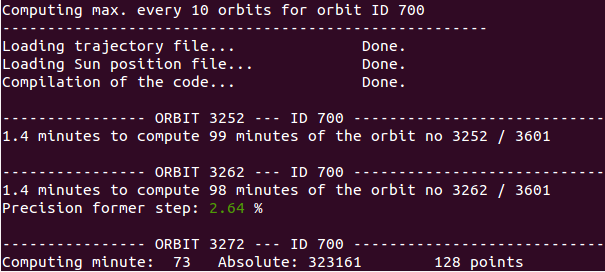
\includegraphics[width=0.7\linewidth]{ex-pipeline}
 \end{center}
\caption{Typical screen output of the pipeline\label{fig:ex-pipeline}}
\end{figure}

\subsection{Running the Analysis Tools}
Once the simulations of the SL contamination are finished, the data must be copied in the folder \verb=<id>_flux/=. The only mandatory module to run is the first one (\verb=2-orbits_computed.py=) as it builds the index of the \emph{effectively} computed orbits. The order proposed in the original pack is increasing in the complexity of the analysis. It first focuses on the parameters of the simulation and testing the robustness of the data. The few last modules analyses the data from the point of view of observation capabilities and prepares the planning of the observations.

All the provided modules contain a documentation at the beginning of the file explaining the purpose of the file, the parameters, requirements, \dots\ Some modules require additional folder to store the output figures, maps or data. The amount of time required for a given module can be quite long and depends on the length of the epoch and usually on the number of orbits computed during the pipeline phase.

\section{Troubleshooting} \label{sec:Troubleshooting}
\subsection{Pipeline}
\begin{description}
 \item [The error is always greater than the threshold] There is a parameter that could influence the error made from one orbit to the next: the parameter \verb=magnitude_max= in \verb=parameters.py= which is used to clip low values of the SL flux. If this number is set too high, then it becomes highly sensitive.
 \item [The pipeline refuses to compile the code] There is a problem of permission for the file\\ \verb=stray_light_<id>/CODE/compile=. Make sure that the CHMOD is configured to 777 for this file. The compilation of the Fortran code necessitate the \verb=gfortran= compiler. The automatic compilation can be turned off in \verb=1-compute-MASTER.py=.
\end{description}
\subsection{Analysis Tools}
\begin{description}
 \item [Python cannot write data file] This should start when you run this error analysis already. The distribution of Numpy may still be lower than 1.7.0. If this is the case, we recommend you install the latest version (downloaded from their website) manually. If this does not fix the issue, make sure that the output directory exists.
  \item [Replacing flux files] For some reason, if some part of the simulations were not done correctly, it may be necessary to replace some of the data. Manipulating the flux files by hand can reveal very tedious. A script was designed to replace a portion of the data. Running 
 \begin{lstlisting}
  python b-replace_flux.py
 \end{lstlisting}
 will move the current data used in the analysis to a trash folder which must \emph{exist} prior to running the code. The new data are copied from the the pipeline folder. See the file itself for the parameters.
\end{description}


\section{Known Issues} \label{sec:KnownIssues}
In this section, the known weakness of the code are presented. User who notice other issues are welcomed to send their comments to the authors.
\begin{itemize}
 \item A constant albedo is used not modelling correctly the surface of the Earth, the weather or the thunders. In the stray light code, the albedo $A$ is taken to be one to yield a worst case scenario. This factor is a multiplicative factor in the computation of the stray light as:
\begin{equation}
 F_\text{sl} = S_V\int_{\Omega({\text{i,s,}\oplus})} A\cos\vartheta\cos\varphi\text{d}\Omega
\end{equation}
where $\Omega({\text{i,s,}\oplus})$ is the illuminated Earth visible from the satellite, $S_V$ the Solar flux in the relevant band, $\vartheta$ the angle LOS--illuminated surface element, $\varphi$ angle direction of Sun--normal of surface element. It can be computed that changing the albedo to an averaged value of 0.35 \citep{Pater2001} would push the limiting magnitude by about 1.1 magnitude fainter. Around the poles however, the albedo is higher due to the ice and the snow (around 0.9) while oceans or continents have a much lower albedo (down to 0.1).
\item PSF, Aperture and Uncertainty. Changing the aperture of the telescope by 1 cm with a constant PSF increases the flux by $\sim13\%$ or a 0.13 mag brighter in the CHEOPS case. To get a more precise value therefore of the equivalent magnitude, a convolution of the signal is to be made. Given a change in what would be the equivalent PSF radius for a top-hat function of $\pm 20\%$ would lead to a change of $^{-0.20}_{+0.25}$ respectively in the magnitude.
 \item The function \verb=compare_two_orbits()= may cause some problems. The cause is that the time 0 in an orbit may not always be located at the same point in the orbit as the period of the orbit is not an integer. The code will try to find the best possible fit by adjusting a shift between the two orbits. It is also sensitive to the parameter \verb=ppm_threshold= set in \verb=parameters.py=.
 \item When drawing images of the stray light on the sky (\verb=9-plot_flux.py=), the function \verb=draw_boundaries()= does not work properly if the observable zone is made up of more than one region.
 \item The script that calculate the almanac of a single target does not work properly. In general, ephemerides calculation from a target catalogue should be considered as beta implementation. 
 \item There might be some unexpected differences (up to 1\% in the total sky coverage) in observability maps as shutdowns of the satellite are not taken into account. This can be explained by the way the observable cells in the sky maps are computed.
\end{itemize}


%%%%%%%%%%%%%%%%%%%%%%%%% BIBLOGRAPHY %%%%%%%%%%%%%%%%%%%%%%%%%%%%
% \newpage
\bibliographystyle{apj}
% \nocite{*}
\bibliography{documentation.bib}
%%%%%%%%%%%%%%%%%%%%%%%%% appendices %%%%%%%%%%%%%%%%%%%%%%%%%%%%
% \newpage
\begin{appendices}
\section{List of Abbreviations} \label{app:abbreviations}
 \begin{table*}[!h]
 \begin{center}
  \begin{tabular}{lp{13.5cm}} \toprule
%    CCD & Charged Coupled Device \\
    CHEOPS & CHaracterizing Exoplanets Satellite \\
    EPFL & Ecole Polytechnique F\'ed\'erale de Lausanne \\
%     ETHZ & Eidgen\"ossische Technische Hochschule Z\"urich \\
%     EChO & Exoplanet Characterisation Observatory \\
    ESA & European Space Agency \\
%     ESO & European Southern Observatory \\
%     FOV & Field Of View \\
%     FWHM & Full Width at Half Maximum \\
%     HARPS & High Accuracy Radial velocity Planetary Search \\
%     HST & Hubble Space Telescope \\
%     IAU & International Astronomical Union \\
%     ICRF & International Celestial Reference Frame \\
    INAF & Istituto Nazionale di Astrofisica / Italian national institute for astrophysics\\
    LEO & Low Earth Orbit \\
    LOS & Line Of Sight \\
%     LTAN & Local Time of the Ascending Node\\
%     MOA & Microlensing Observations in Astrophysics \\
%     NASA & National Aeronautics and Space Administration \\
%     OGLE & Optical Gravitational Lensing Experiment \\
%     ppm & Parts per million \\
%     PSF & Point Spread Function \\
    PST & Point Source Transmittance function \\
%     RAAN & Right Ascension of the Ascending Node \\
%     RMS & Root mean square \\
%     RV & Radial Velocity detection technique \\
    SAA & South Atlantic Anomaly \\
%     S/C & Spacecraft \\
%     SDSS & Sloane Digital Sky Survey \\
    SL & Stray Light \\
    SNR & Signal-to-Noise Ratio \\
%     SSO & Sun-Synchronous Orbit \\
%     TAPS & Theoretical Astrophysical and Planetary Science Group at UniBe\\
%     TESS & Transiting Exoplanet Survey Satellite\\
     Unibe & University of Bern \\
%     UniGe & University of Geneva \\
   \bottomrule
  \end{tabular}
  \end{center}
\end{table*}
\end{appendices}

\end{document}
